% !TeX root = main.tex
\section{A First Example: Computing a Barcode (Part two)}

Recall the Hamiltonian diffeomorphism
\begin{equation}
\phi(x,y) = ( x + a \sin(y + a \sin(x)), y + a \sin(x)),
\end{equation}
with $a > 0$, whose fixed points are $(0,0)$, $(0,\pi)$, $(\pi, 0)$ and $(\pi,\pi)$. We will now compute the filtered Floer homology of $\phi$.

First, we compute the Maslov index of these fixed points, using a slightly modified version of the algorithm from page \pageref{page:maslovalg}. The essential insight is that the torus admits a global frame, so the choice of smooth functions $Z_i(x)$ is unnecessary: We have a default way to write $(\dl \phi_t)_x$ as a matrix.

We present the simplified algorithm to compute the Maslov index in a manifold admitting a global frame.
\begin{enumerate}[algorithm]\label{page:maslovalg2}
\item Consider the linear map $(\dl \phi_t)_x$. Using the global matrix, represent it as a matrix $A(t)$.
\item Compute the Conley-Zehnder index of the path $A(t)$.
\end{enumerate}

To proceed, we should compute $(\dl \phi_t)_{(x,y)}$ in matricial form. Recall that $\phi_t$ is the flow of the smooth Hamiltonian $H_1$, which is a smoothed version of the Hamiltonian
\begin{equation}
H_0(x,y,t) = \begin{cases}
-\cos(x), & t < a,\\
\cos(y), & t > a.
\end{cases}
\end{equation}

The smoothing hypothesis is necessary for theoretical reasons, but for practical computations it is actually unnecessary, as it merely corresponds to a reparametrization of the flow. Therefore, in the computations that follow, we will be surreptitiously working with the flow of $H_0$ instead of the flow of $H_1$, as the computations become a lot more bearable.

The flow of $H_0$ is written as
\begin{equation}
\phi_t(x,y) = \begin{cases}
(x,y+t \sin(x)), & 0 \leq t \leq a,\\
(x+t \sin(y+a \sin(x)), y + a \sin(x)), & a \leq t \leq 2a.
\end{cases}
\end{equation}

The derivative of $\phi_t$ can be likewise written by cases
\begin{equation}\label{dphi1}
A(t) := (\dl \phi_t)_{(x,y)} = \begin{cases}
\begin{bmatrix}
1 & 0\\
t \cos(x) & 1
\end{bmatrix} & 0 \leq t \leq a,\\[1.3em]
\begin{bmatrix}
\scalebox{0.7}{$1+(t-a) a \cos(y+a \sin(x)) \cos(x)$} &  (t-a) \cos(y)\\
a \cos(x) & 1
\end{bmatrix}
 & a \leq t \leq 2a.
\end{cases}
\end{equation}

At this point, it should be obvious that the notation is becoming burdensome, so we present a clearer way to write paths of matrices such as \eqref{dphi1}.

Here and in the rest of this article, we will use the following notation for such a path of matrices.
\begin{equation}\label{rectpath}
A(t) :
\begin{bmatrix}
1 & 0\\
0 & 1
\end{bmatrix}
\to
\begin{bmatrix}
1 & 0\\
a \cos(x) & 1
\end{bmatrix}
\to
\begin{bmatrix}
\scalebox{0.7}{$1+ a^2 \cos(y+a \sin(x)) \cos(x)$} &  a \cos(y)\\
a \cos(x) & 1
\end{bmatrix}
\end{equation}

The notation of \eqref{rectpath} is intended to suggest a rectilinear path, where each arrow represents a section being linearly interpolated.

For $(x,y)$ a fixed point of the flow of $H_0$, $\sin(x) = \sin(y) = 0$ and the cosines evaluate to $\pm 1$, and therefore \ref{rectpath} becomes
\begin{equation}\label{rectpath1}
A(t):
\begin{bmatrix}
1 & 0\\
0 & 1
\end{bmatrix}
\to
\begin{bmatrix}
1 & 0\\
\pm_1 a & 1
\end{bmatrix}
\to
\begin{bmatrix}
1 \pm_1 \pm_2 a^2 &  \pm_2 a\\
\pm_1 a & 1
\end{bmatrix}
\end{equation}
where $\pm_1 1$ is $1$ if $x=0$ and $-1$ if $x = \pi$, and likewise for $\pm_2 1$ and $y$.

To compute the Conley-Zehnder index of \eqref{rectpath1}, let us begin by looking at the trace of $A(t)$, specifically in the easy case where $\pm_1 \pm_2 1 = +1$. In this case, $\trace A(t)$ follows the piecewise rectilinear path
\begin{equation}
\trace A(t) : 2 \to 2 \to 2 + a^2,
\end{equation}
which starts at $2$ and ends at a value greater than $2$. Therefore, $\rho(A(t))$ is constant equal to 1, and its winding number is null.\footnote{Technically we should instead work with an extension of $A(t)$ which ends at $W^-$. However, such an extension $\tilde A$ would be entirely contained in $Sp(2)^-$ and therefore $\rho \circ \tilde A$ would also be constant equal to 1.} Consequently, using obvious notation to denote the Maslov index of periodic orbits,
\begin{equation}
\mu(0,0) = \mu(\pi,\pi) = 0.
\end{equation}

We now turn to the case $\pm_1 \pm_2 1 = -1$. In this case,
\begin{equation}
\trace A(t) : 2 \to 2 \to 2 - a^2.
\end{equation}

The first step is to extend $A$ to a path ending in $W^+$, per corollaries \ref{sp2sgn} and \ref{sp2pm}. To the resulting path we would like to apply proposition \ref{calcmaslov}, but there is one obstacle: In the resulting decomposition $0 = a_0 < b_0 < a_1 = T$, we might not know \textit{a priori} what $A(b_0)$ looks like, because $b_0$ might lie outside the domain where the extension agrees with $A$. We will discuss how to get around this issue shortly, but first we will deal with the easy case where this is not a problem.

[Maybe rephrase this because we already did such an example, kind of, in the autonomous case]

\begin{prop}\label{easymaslov}
Let $A(t)$, $t \in \interval02$, be the path
\begin{equation}
A(t):
\begin{bmatrix}
1 & 0\\
0 & 1
\end{bmatrix}
\to
\begin{bmatrix}
1 & 0\\
\pm a & 1
\end{bmatrix}
\to
\begin{bmatrix}
1 - a^2 &  \mp a\\
\pm a & 1
\end{bmatrix},
\end{equation}
where the linear interpolation has nodes at $0$, $1$ and $2$.

Then, if $a \geq \sqrt2$, the Maslov index of $A$ is equal to $\mp 1$.
\end{prop}

\begin{proof}
Let $\tilde A(t)$, $t \in \interval03$, be an extension of $A$ such that $\tilde A(3) = W^+$ and $\trace \tilde A(t) < 2$ for $t \in \interval23$. Apply proposition \ref{calcmaslov} to the path $\tilde A$, using the partition
\begin{equation}
a_0 = 0, b_0 = 1 + \frac2{a^2}, a_1 = 3.
\end{equation}

Note: It is here that we use the hypothesis that $a \geq \sqrt2$, as otherwise the value of $b_0$ would be greater than $2$ and be in a section of $\tilde A$ over which we have no control.

The verification that we are in the hypothesis of proposition \ref{calcmaslov} is mostly trivial, the most difficult property to check being \ref{calcmaslov:ab4}, i.e. that between any two points where one has trace in $\rinterval2\infty$ and the other has trace in $\linterval{-\infty}{-2}$ there exists a value of $b$, which in our case must be $b_0$. This is checked directly by evaluating at which points the trace may take such values.

To compute the Maslov index, we apply formula \eqref{calcmaslov:mu}, still from proposition \ref{calcmaslov}, which tells us that
\begin{equation}\label{easymaslov:eq1}
\mu(\tilde A(t)) = \sign(\tilde A(b_0)_{12}).
\end{equation}

Since the Maslov index of $A$ coincides with the Maslov index of $\tilde A$, it suffices to compute the right-hand side of \eqref{easymaslov:eq1}. Note that
\begin{equation}
\tilde A(b_0) = A(b_0) = 
\begin{bmatrix}
1 & 0\\
\pm a & 1
\end{bmatrix}
+
\frac2{a^2}
\begin{bmatrix}
- a^2 &  \mp a\\
0 & 0
\end{bmatrix}
=
\begin{bmatrix}
-1 & \mp \frac2a\\
\pm a & 1
\end{bmatrix}.
\end{equation}

From this expression we may read off the sign of the element at index $12$, and hence conclude the result.
\end{proof}

To correct the deficiency of proposition \ref{easymaslov}, there are two expedite solutions. One of them would be to build the extension $\tilde A$ explicitly and do the corresponding computations. A second, easier way, is to exploit the independence of the Maslov index on the extension. It is this approach that we will take.

\begin{prop}
Proposition \ref{easymaslov} also holds if $0 < a < \sqrt2$.
\end{prop}

\begin{proof}
The proof is exactly the same, but we modify the construction of $\tilde A$ slightly. First, we extend $A$ by continuing linear interpolation up to time $b_0 = 1 + \frac2{a^2} > 2$, that is,
\begin{equation}
\tilde A(t) = \begin{bmatrix}
1 & 0\\
\pm a & 1
\end{bmatrix}
+
(t-1)
\begin{bmatrix}
- a^2 &  \mp a\\
0 & 0
\end{bmatrix}, \; t \in \interval1{1+\frac2{a^2}}.
\end{equation}

Then we finish the extension by connecting the end of the resulting path to $W^+$.

The rest of the proof follows exactly as in proposition \ref{easymaslov}.
\end{proof}

Since we know the contractible orbits of $H_1$ and their Maslov indices, we know the vector spaces of the filtered Floer complex of $H_1$.

[This part could use some improvement.]

These vector spaces are parametrized by $\lambda \in \R$, the maximum value allowed for the action functional. They also have persistence homology structure induced by the inclusion, so we may represent them via barcodes. This is a much more concise way to represent these spaces, so in the future we will resort to barcodes for such descriptions. In this case, we will also exhibit a description `in words', for comparison.

We will also introduce new notation here: the concept of named bars. The idea is that (recall definition \ref{def:pmfrombarcode}) to each bar of the barcode associated to the vector spaces of the filtered Floer complex corresponds a generator of said vector spaces, i.e. a periodic orbit (or linear combination thereof). Therefore, we may associate to each bar a periodic orbit (or linear combination), which associates to it an element of the basis it may represent. Note that this choice of association is not unique in general.

\begin{prop}
The Hamiltonian $H_1$ has four periodic contractible orbits (in time $2a$), which are represented in the following figure, as well as the corresponding actions and Maslov indices.
\begin{figure}[H]
\centering
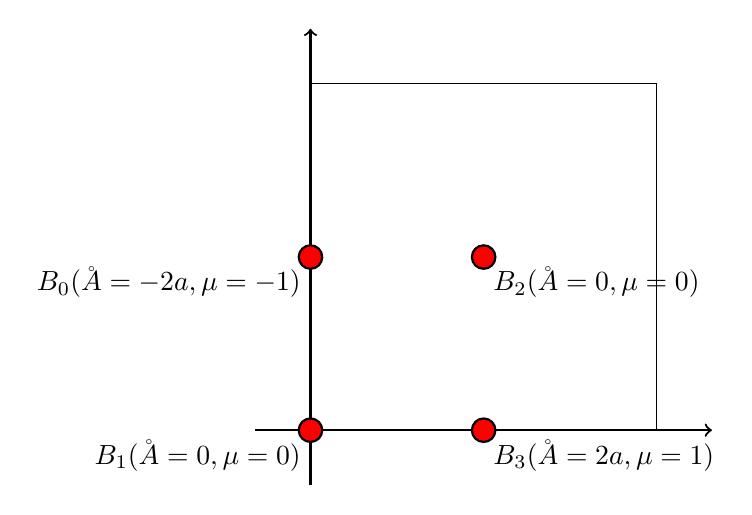
\begin{tikzpicture}[scale=0.7, vertex/.style={draw,circle,thick,fill=red,inner sep=3pt}]
\draw[->,thick] (-1,0) -- (2*pi+1,0);
\draw[->,thick] (0,-1) -- (0,2*pi+1);
\draw (0,0) rectangle (2*pi,2*pi);

\draw (0,0) node[vertex] {} node[below left] {$B_1 (\AA = 0, \mu = 0)$};
\draw (0,pi) node[vertex] {} node[below left] {$B_0 (\AA = -2a, \mu = -1)$};
\draw (pi,0) node[vertex] {} node[below right] {$B_3 (\AA = 2a, \mu = 1)$};
\draw (pi,pi) node[vertex] {} node[below right] {$B_2 (\AA = 0, \mu = 0)$};
\end{tikzpicture}
\caption{The periodic orbits of $H_1$ and their actions and Maslov indices}
\label{orbitsh1}
\end{figure}

Consequently, the vector spaces of the Floer complex are given by
\begin{equation}
\begin{gathered}
\CF_{-1}^\lambda(H_1) = \begin{cases}
0, & \lambda \leq -2a,\\
\braket{B_0} & \lambda > -2a,
\end{cases}
\\
\CF_{0}^\lambda(H_1) = \begin{cases}
0, & \lambda \leq 0,\\
\braket{B_1,B_2} & \lambda > 0,
\end{cases}
\\
\CF_{1}^\lambda(H_1) = \begin{cases}
0, & \lambda \leq 2a,\\
\braket{B_3} & \lambda  > 2a.
\end{cases}
\end{gathered}
\end{equation}

This information can be sumarily represented via the following barcode.
\begin{figure}[H]
\centering
\begin{tikzpicture}
\draw[->,thick] (-4.500,0.000)--(4.500,0.000);
\draw[] (0.000,-0.200)--(0.000,0.200) node[above] {0};
\draw[] (2.500,-0.200)--(2.500,0.200) node[above] {$2a$};
\draw[] (-2.500,-0.200)--(-2.500,0.200) node[above] {$-2a$};
\draw[(-,thick] (-2.500,-0.500)--(4.200,-0.500) node[right] {$B_0$};
\node[] at (5.500,-0.500) {$(\CF_{-1})$};
\draw[(-,thick] (0.000,-1.100)--(4.200,-1.100) node[right] {$B_1$};
\draw[(-,thick] (0.000,-1.500)--(4.200,-1.500) node[right] {$B_2$};
\node[] at (5.500,-1.300) {$(\CF_0)$};
\draw[(-,thick] (2.500,-2.100)--(4.200,-2.100) node[right] {$B_3$};
\node[] at (5.500,-2.100) {$(\CF_1)$};
\end{tikzpicture}
\caption{The barcode of the filtered Floer complex of $H_1$}
\end{figure}
\end{prop}

All that remains is to compute the boundary maps $\partial$. By using the fact that Floer homology must coincide with Morse homology (as $\lambda \to \infty$) it is easy to conclude that these boundary maps must be null, but in order to illustrate a method which will be useful later we will show directly that they are null by exploiting symmetries of the space $M$ and the Hamiltonian $H_1$.

\subsection{Symmetries}

We begin by recalling the definition of $\partial(b)$, where $b$ is a periodic orbit of $H_1$. First, one must compute the Maslov index $\mu(b)$. Then, $\partial(b)$ will be of the form
\begin{equation}
\partial(b) = \sum n(b,c) c,
\end{equation}
where the sum is taken over orbits $c$ whose Maslov index is $\mu(c) = \mu(b)-1$. The numbers $n(b,c)$ are computed by counting how many pseudo-holomorphic curves connect $b$ and $c$. A pseudo-holomorphic curve is a $C^\infty$ function $(x(t,s), y(t,s))$, $t \in \R / T$, $s \in \R$, satisfying
\begin{equation}\label{pseudoholomorphic}
\begin{cases}
\displaystyle \diffp x s - \diffp y t = \diffp H x(x,y,t),\\[1em]
\displaystyle \diffp y s + \diffp x t = \diffp H y(x,y,t).
\end{cases}
\end{equation}

We say that such a curve $(x,y)$ connects the periodic orbits $b$ and $c$ if the following limits hold in the $C^\infty$ sense
\begin{equation}
\lim_{s \to -\infty} (x,y)(t,s) = b(t), \; \lim_{s \to \infty} (x,y)(t,s) = c(t).
\end{equation}

The set of such solutions, modulo translation of $s$, is denoted $\moduli(b,c)$.

Now, we are only interested in the number of said curves modulo 2, so if we find any symmetries in $\moduli(b,c)$ in the form of an involution $F \colon \moduli(b,c) \to \moduli(b,c)$ we will only need to examine solutions which are symmetrical, i.e. $F(u) = u$. In our case, such involutions will come from well-chosen changes of variable.

For example, suppose we wish to compute $n(B_3, B_1)$ (see figure \ref{orbitsh1}). The key is the axis of symmetry of the torus about the vertical line $x = \pi$. In other words, if $(x,y)(t,s)$ is a pseudo-holomorphic orbit connecting $B_3$ to $B_1$, i.e. an orbit of $\moduli(B_3,B_1)$, it is reasonable to conjecture that the orbit $(2\pi-x, y)(t,s) = (-x,y)(t,s)$ is also in $\moduli(B_3,B_1)$.

The first thing that needs to be checked is that the $C^\infty$ limits as $s \to \pm \infty$ still coincide with $B_1$ and $B_3$. This is a trivial check, as the reflection about $x = \pi$ preserves the $C^\infty$ norm, as well as the orbits $B_1$ and $B_3$. Therefore, it suffices to check the pseudo-holomorphicity of the orbit $(-x,y)(t,s)$. Unfortunately, this is where we run into problems, because, in general,
\begin{equation}
\label{nottrue1}
\begin{cases}
\displaystyle \diffp{(-x)} s - \diffp y t = \diffp H x(-x,y,t),\\[1em]
\displaystyle \diffp y s + \diffp{(-x)} t = \diffp H y(-x,y,t)
\end{cases}
\text{ is \emph{not} true!}
\end{equation}

In order to correct and prove a statement similar to \eqref{nottrue1}, it is first useful to consider what can be said about $\grad_{x,y} H(x,y,t)$. To do so, we investigate symmetries of $H_t$ in space (and eventually in time) and see how they are reflected in symmetries of $\grad_{x,y} H$.

For example, the Hamiltonian $H_0(x,y,t)$, as well as its smoothing $H_1$, satisfies the symmetry
\begin{equation}
H(-x,y,t) = H(x,y,t).
\end{equation}

Consequently, taking partial derivatives, we obtain the symmetries
\begin{equation}\label{eq:symmetries1}
- \diffp H x(-x,y,t) = \diffp H x(x,y,t),\quad \diffp H y(-x,y,t) = \diffp H y (x,y,t).
\end{equation}

This points to how \eqref{nottrue1} might be fixed. For example, the right-hand side of the second equation of \eqref{nottrue1} equals
\begin{equation}
\diffp H y (-x,y,t) = \diffp H y (x,y,t) \stackrel{\text{$(x,y)$ pseudo-holom.}}{=} \diffp y s + \diffp{x} t,
\end{equation}
and the last term is not equal to $\diffp y s + \diffp{(-x)} t$ by a factor of $-1$ in the second term. An easy way to correct this factor is to swap the variable $t$ for $-t$. This creates another problem, because $H(-x,y,-t) \neq H(x,y,t)$, but a translation in time yields the symmetry
\begin{equation}
H(-x,y,a - t) = H(x,y,t).
\end{equation}

Therefore, \eqref{eq:symmetries1} can be modified to yield the slightly different symmetries
\begin{equation}
- \diffp H x(-x,y,a-t) = \diffp H x(x,y,t),\quad \diffp H y(-x,y,a-t) = \diffp H y (x,y,t).
\end{equation}

This finally allows us to define the involution. Given an orbit $(x,y)(t,s) \in \moduli(B_3,B_1)$, define
\begin{equation}
(\tilde x, \tilde y)(t,s) = (-x,y)(a-t,s).
\end{equation}

We verify that $(\tilde x, \tilde y) \in \moduli(B_3, B_1)$.
\begin{itemize}
\item The conditions at infinity are verified because the operator $(x,y)(t) \mapsto (-x,y)(a-t)$ preserves $C^\infty$ norm and the constant orbits $B_3$ and $B_1$.

\item The curve $(\tilde x, \tilde y)$ is pseudo-holomorphic, as can be checked directly. As an example, we verify the first equation in \eqref{pseudoholomorphic}; the second equation is verified analogously.

\begin{equation}
\begin{aligned}
\diffp{\tilde x}s - \diffp{\tilde y}t &= \diffp{(-x)(a-t,s)}s - \diffp{y(a-t,s)}t\\
&= - \diffp x s(a-t, s) + \diffp y t(a-t, s)\\
&= - \diffp H x (x(a-t,s), y(a-t,s), a-t)\\
&= \diffp H x (\tilde x(t, s), \tilde y(t, s), t).
\end{aligned}
\end{equation}
\end{itemize}

This proves that the involution $(x,y) \mapsto (\tilde x, \tilde y)$ maps elements of $\moduli(B_3,B_1)$ to itself, so modulo 2 we need only count solutions which are symmetric with regard to this involution. We will now show that there are no such solutions.

If $(x,y) = (\tilde x, \tilde y)$, note that $x(\tfrac a 2, s) = - x(\tfrac a 2, s)$ in the torus, i.e. modulo $2\pi$. Therefore,
\begin{equation}
x(\tfrac a 2, s) \in \{0,\pi\}, \mod 2\pi.
\end{equation}

Now, as $s \to -\infty$ this quantity must converge to $\pi$ and as $s \to \infty$ this quantity converges to $0$. This is a contradiction, because the space of possible values in which $x(\tfrac a 2, s)$ may be in is discrete, and since this quantity is continuous in $s$ it must be constant. Therefore, there are no symmetric solutions, and $n(B_3, B_1) = 0$.

The same symmetry shows that $n(B_2, B_0) = 0$, and a similar argument with the variable change
\begin{equation}
x \to x, y \to -y, t \to a-t,
\end{equation}
shows that the other values of $n$ are also null. This completes the proof of

\begin{prop}
The boundary maps of the filtered Floer complex of $H_1$ are all null. Consequently, the barcode of its time-$2a$ flow coincides with the barcode of the Floer complex of $H_1$, which is represented in the following figure.

\begin{figure}[H]
\centering
\begin{tikzpicture}
\draw[->,thick] (-4.500,0.000)--(4.500,0.000);
\draw[] (0.000,-0.200)--(0.000,0.200) node[above] {0};
\draw[] (2.500,-0.200)--(2.500,0.200) node[above] {$2a$};
\draw[] (-2.500,-0.200)--(-2.500,0.200) node[above] {$-2a$};
\draw[(-,thick] (-2.500,-0.500)--(4.200,-0.500) node[right] {$B_0$};
\node[] at (5.500,-0.500) {$(\HF_{-1})$};
\draw[(-,thick] (0.000,-1.100)--(4.200,-1.100) node[right] {$B_1$};
\draw[(-,thick] (0.000,-1.500)--(4.200,-1.500) node[right] {$B_2$};
\node[] at (5.500,-1.300) {$(\HF_0)$};
\draw[(-,thick] (2.500,-2.100)--(4.200,-2.100) node[right] {$B_3$};
\node[] at (5.500,-2.100) {$(\HF_1)$};
\end{tikzpicture}
\caption{The barcode of the time-$2a$ flow of $H_1$.}
\end{figure}

\end{prop}